
\documentclass[10pt]{article} % For LaTeX2e
\usepackage[preprint]{tmlr}
% If accepted, instead use the following line for the camera-ready submission:
%\usepackage[accepted]{tmlr}
% To de-anonymize and remove mentions to TMLR (for example for posting to preprint servers), instead use the following:
%\usepackage[preprint]{tmlr}

% Optional math commands from https://github.com/goodfeli/dlbook_notation.
\input{math_commands.tex}

\usepackage{hyperref}
\usepackage{url}
\usepackage{graphicx}
\usepackage{longtable}
\usepackage{booktabs}
\usepackage{csvsimple}

\usepackage[none]{hyphenat}
\sloppy


\title{Universal Compression Scaling Laws Across Modalities}

% Authors must not appear in the submitted version. They should be hidden
% as long as the tmlr package is used without the [accepted] or [preprint] options.
% Non-anonymous submissions will be rejected without review.

\author{\name Aryasomayajula Ram Bharadwaj \thanks{%
Equal contribution. This research was conducted as part of an EleutherAI community project that began in July 2025.}
      \email ram.bharadwaj.arya@gmail.com \\
      \addr Independent Researcher
      \AND
      \name Edric Castel C. Hao \footnotemark[1] \email edric.hao@gmail.com \\
      \addr Independent Researcher}

% The \author macro works with any number of authors. Use \AND 
% to separate the names and addresses of multiple authors.

\newcommand{\fix}{\marginpar{FIX}}
\newcommand{\new}{\marginpar{NEW}}

\def\month{February}  % Insert correct month for camera-ready version
\def\year{2026} % Insert correct year for camera-ready version
\def\openreview{\url{https://openreview.net/forum?id=XXXX}} % Insert correct link to OpenReview for camera-ready version


\begin{document}


\maketitle

\begin{abstract}
We establish empirical scaling laws for the compression capabilities of large language models across four modalities: text, image, speech, and scene graphs. Using Pythia transformer models ranging from 70M to 12B parameters across five training checkpoints, we demonstrate that compression ratio exhibits robust power-law dependence on both model size and training progress across multiple modalities. Our key finding is that compression ratio $\mathrm{CR}(P,S)$ can be accurately modeled as:
\[
\mathrm{CR}(P,S) = a + b P^{-\alpha} + c S^{-\beta}
\]
where $P$ is the number of parameters and $S$ is the training step. We demonstrate that this scaling behavior is consistent across multiple modalities. While genomic sequences do not exhibit a clear monotonic scaling trend with respect to model size or training progress, their absolute compression ratios fall within a systematic ordering across modalities. In particular, text achieves the highest compression efficiency, followed by scene graphs, genomic sequences, speech, and images.
\end{abstract}

\section{Introduction}

The fundamental connection between prediction and compression, established by Shannon's source coding theorem \citep{shannon1948mathematical}, has gained renewed relevance with the rise of large language models (LLMs). Recent work by \citet{deletang2024compression} demonstrated that LLMs can serve as powerful general-purpose compressors, while \citet{kaushik2023llmzip} showed state-of-the-art text compression using LLaMA with arithmetic coding. However, a systematic understanding of how compression performance scales with model size and training progress across different modalities remains unexplored.

This work fills that gap by establishing empirical scaling laws for LLM-based compression. We conduct the first comprehensive study of compression scaling across text, image, speech, scene graph, and genomic sequence modalities using Pythia models \citep{biderman2023pythia} ranging from 70M to 12B parameters. Our main contributions are:

\begin{enumerate}
\item \textbf{Universal Scaling Laws}: We demonstrate that compression ratio follows predictable power laws in model parameters $P$ and training steps $S$ across most modalities.
\item \textbf{Cross-Modal Analysis}: We show how scaling varies between text, image, speech, scene graphs, and genomic sequences revealing modality-specific compression dynamics.
\item \textbf{Theoretical Connection}: We establish the link between our compression scaling laws and Hoffman et al.'s cross-entropy scaling, providing theoretical grounding for our empirical observations.

\item \textbf{Practical Implications}: Our results enable prediction of compression performance and optimal resource allocation for compression-focused applications.
\end{enumerate}

\section{Background and Related Work}
\subsection{Compression and Prediction Equivalence}

The connection between prediction and compression is fundamental to information theory. For any probabilistic model $p_\theta$, arithmetic coding achieves compression with expected code length approaching the cross-entropy $H(p_{data}, p_\theta) = \mathbb{E}_{x \sim p_{data}}[-\log_2 p_\theta(x)]$. This establishes the compression ratio as:
\[
\mathrm{CR} = \frac{\text{compressed bits}}{\text{original bits}} = \frac{H(p_{data}, p_\theta)}{H(p_{data})} = 1 + \frac{\mathrm{KL}(p_{data} \parallel p_\theta)}{H(p_{data})}
\]

Thus, better predictive models (lower KL divergence) achieve better compression ratios, creating a direct link between language modeling performance and compression capability.

\subsection{Scaling Laws for Language Models}

\citet{kaplan2020scaling} established that language model performance follows power laws:
\[
L(N) = \left(\frac{N_c}{N}\right)^{\alpha_N}, \quad L(D) = \left(\frac{D_c}{D}\right)^{\alpha_D}, \quad L(C) = \left(\frac{C_c}{C}\right)^{\alpha_C}
\]
where $L$ is cross-entropy loss, $N$ is model size, $D$ is dataset size, and $C$ is compute. The exponents $\alpha_N \approx 0.076$, $\alpha_D \approx 0.095$, and $\alpha_C \approx 0.050$ for text modeling.

\citet{hoffmann2022scaling} modified the functional form based on risk decomposition to include an asymptotic error term equivalent to the loss if given infinite data and compute budget:
\[
L(N, D) = E + \frac{A}{N^\alpha} + \frac{B}{D^\beta}
\]
where E is an estimate of the entropy of natural text, A is the coefficient for scaling model size, and B is the coefficient for scaling dataset size.

In subsequent years, multiple studies have sought to identify scaling laws across a variety of modalities, tasks, and architectures. \citet{li2025scaling} surveyed over 50 papers to identify the primary power-law forms and examine how choices in model architecture, training regimes, dataset size, evaluation metrics, and fitting procedures affect the resulting scaling laws. They find that most power laws are still based on or adapted from \citet{kaplan2020scaling} or \citet{hoffmann2022scaling}. The number of data points used to fit a scaling law is either unspecified or relatively small due to a limited total compute budget for all experiments. They range from 4 to several hundred data points, with model sizes spanning from roughly 10 million to about 7 billion parameters. However, most studies are limited to fewer than 50 data points and model sizes below 1 billion parameters.

\citet{li2025scaling} also train 11 models with parameter counts ranging from 12 million to 1 billion, using 1-10 checkpoints per model across three datasets, in an effort to replicate the scaling laws of \citet{kaplan2020scaling} and \citet{hoffmann2022scaling}. \citet{pearce2024scaling} attempt to reconcile these two laws through a small-scale study with 5 model sizes and 6 training token budgets on the BookCorpus dataset. \citet{hu2024scaling} show that stable checkpoints remove the need to retrain models from scratch and fit scaling curves using SciPy’s curve\_fit function across 6 models ranging from 40 million to 2 billion parameters with 6 checkpoints per model. These studies reveal consistent scaling trends across tasks and datasets despite the limited number of data points imposed by compute budgets.


\subsection{LLM-Based Compression}

\citet{deletang2024compression} showed that large language models can compress data across modalities using arithmetic coding, achieving better compression than specialized algorithms like PNG for images and FLAC for audio. \citet{kaushik2023llmzip} demonstrated state-of-the-art text compression using LLaMA-7B with arithmetic coding, achieving compression ratios of 0.71 bits/character on text8. \citet{pandey2024compression} discovered that training-loss scaling behavior varies with dataset compressibility by fitting regression lines between each dataset’s gzip compression ratio and its own set of five training-loss scaling parameters.

\citet{li2024llmzip} propose data compression as an evaluation metric due to its correlation with generalization ability as an alternative to benchmarks affected by data contamination. They find that the performance of large language models degrades on data beyond the training cutoff date and that these models struggle with compressing multimodal data. \citet{zhang2025llmzip} attempt to address this limitation by applying transform coding prior to tokenization, but their comparisons are restricted to outdated compression algorithms. These works suggest that compression captures meaningful aspects of generalization, yet existing analyses remain fragmented, focusing on fixed model scales, isolated modalities, or static training checkpoints. As a result, no prior work has systematically studied how compression performance scales with model size and training progress across multiple modalities.

\section{Methodology}
\subsection{Models and Training}

We use the Pythia model family \citep{biderman2023pythia}, which provides models trained with identical data and hyperparameters across different scales. We evaluate eight model sizes: 70M, 160M, 410M, 1B, 1.4B, 2.8B, 6.9B, 12B non-embedding parameters. For each model size, we use five training checkpoints: 1,000, 8,000, 32,000, 128,000, and 143,000 steps, providing 40 model-checkpoint combinations per modality. To assess whether compression performance is broadly comparable across model families, we additionally evaluate the fully trained OLMo-1B and OLMo-7B models as reference points.

\subsection{Datasets}

We evaluate compression across six data modalities using established benchmarks alongside a synthetic uniformly random baseline for control:
\begin{itemize}
\item \textbf{Text}: enwik8 - Wikipedia XML compression benchmark
\item \textbf{Image}: ImageNet patches - 32×64 grayscale image patches  
\item \textbf{Speech}: LibriSpeech - 16kHz English speech audio
\item \textbf{Scene Graph}: Visual Genome - subject-relationship-object triples
\item \textbf{Genomic Sequence}: Chromosome 22 - nucleotide sequence from the GRCh38 human reference genome

\end{itemize}

For each modality, we create datasets of 2,048 chunks, each containing exactly 2,048 bytes, ensuring fair comparison across modalities.

\subsection{Compression Protocol}

We implement arithmetic coding using model token probabilities following \citet{deletang2024compression}. The compression process:

\begin{enumerate}
\item Convert raw bytes to ASCII text (handling non-ASCII bytes by bit shifting)
\item Tokenize using the model's tokenizer (SentencePiece with 50K vocabulary)
\item For each token position, compute $-\log_2 p_\theta(\text{token}|\text{context})$
\item Sum log-probabilities to get total compressed bits
\item Compute compression ratio: $\mathrm{CR} = \frac{\text{compressed bits}}{2048 \times 8}$
\end{enumerate}

\section{Results}

\subsection{Experimental Data}

Our comprehensive evaluation across 200 model–checkpoint–modality combinations reveals clear scaling behavior in text, speech, image, and scene graph modalities. Figure~\ref{fig:scaling_laws} illustrates the relationship between compression ratio, model parameters, and training steps across these modalities. The complete experimental results for each modality are provided in Appendix~\ref{appendix:experimental_data}. Out-of-sample scaling is evident for most modalities, although the fit is slightly weaker for text and scene graphs ($R^2 \approx 0.87\text{--}0.89$), despite LLMs being primarily trained on textual data. In contrast, speech and images exhibit very strong out-of-sample fits ($R^2 > 0.95$). Interestingly, genomic sequences do not exhibit systematic scaling, highlighting modality-dependent differences in compression behavior.

\begin{figure}[!b]
\centering
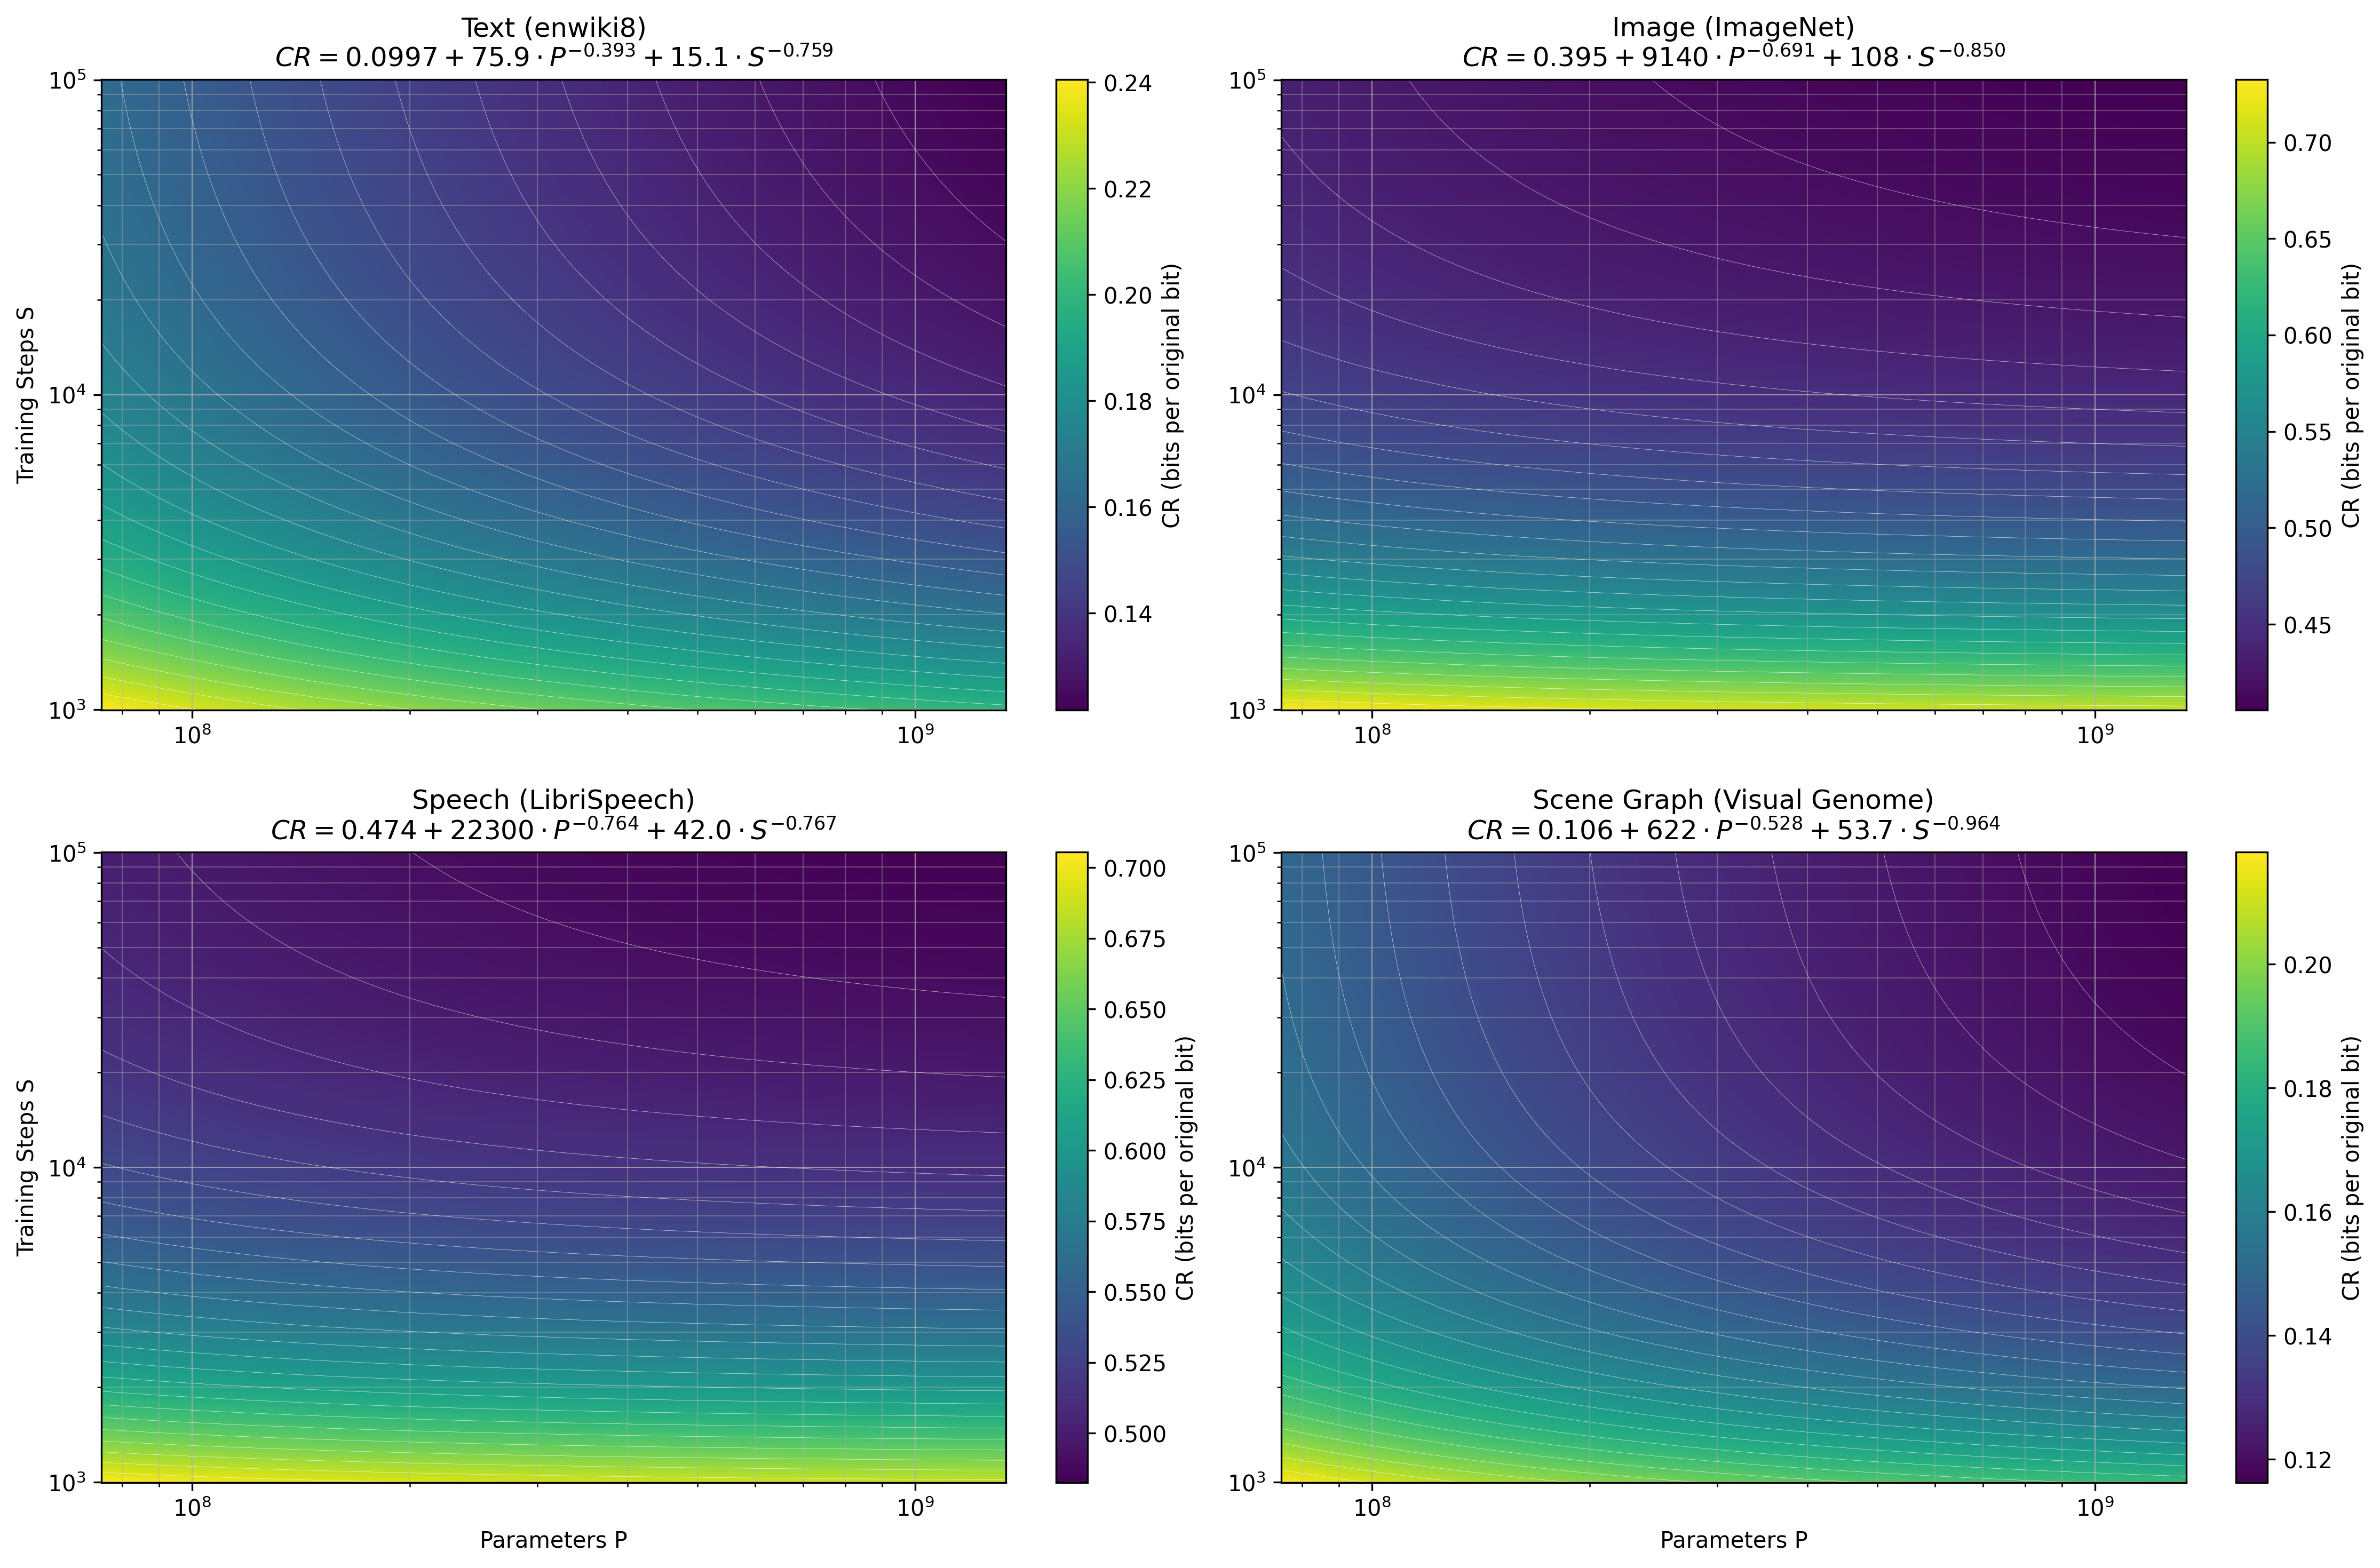
\includegraphics[width=\textwidth]{scaling_laws.png}
\caption{Scaling laws for LLM compression across text, image, speech, and scene graph modalities. The heatmaps show compression ratio as a function of model parameters (P) and training steps (S). Lower compression ratios (darker colors) indicate better compression performance. Each modality follows the power law $\mathrm{CR}(P,S) = a + bP^{-\alpha} + cS^{-\beta}$ with modality-specific coefficients shown in the equations above each subplot.}
\label{fig:scaling_laws}
\end{figure}

\subsection{Experimental Observations}

The experimental results reveal several key patterns across modalities:

\textbf{Model Size Effects}: Across four modalities, larger models consistently achieve better compression ratios. For text (see Appendix Table~\ref{tab:text_results}), the compression ratio improves from approximately 0.22 (70M parameters) to 0.10 (12B parameters) at the final checkpoint. Similar trends are observed for images, speech, and scene graphs, though with different baseline compression levels.

\begin{figure}[!t]
\centering
\includegraphics[width=\textwidth]{merged_plots.jpeg}
\caption{Scaling trends in compression ratio as a function of model parameters across five training step sizes for each modality. The panels show in-sample points used to fit the scaling curve and out-of-sample points used to evaluate predictive performance. Overlaid are the in-sample and out-of-sample regression lines, illustrating changes in trend as training progresses. The predicted scaling curve for each modality is shown with a 95\% confidence interval computed via the delta method, providing a visual assessment of uncertainty in the scaling law fits.}
\label{fig:scaling_plots}
\end{figure}

\textbf{Training Progress}: Four modalities show improvement with training steps, but the rate of improvement varies. Text and scene graphs shows the most dramatic improvement during early training, while speech and images exhibit more gradual but sustained improvements throughout training.

\textbf{Cross-Modal Baseline Performance}: Text achieves the best absolute compression ratios ($\approx$0.101-0.224), followed by scene graphs ($\approx$0.103-0.218), genomic sequences ($\approx$0.158-0.335), speech ($\approx$0.369-0.771), and images ($\approx$0.453-0.748). This ordering reflects the fundamental compressibility of each modality, with discrete symbolic data exhibiting higher low-order redundancy than continuous signals. However, this baseline hierarchy does not translate directly into scaling behavior. Text and scene graphs, while highly compressible at baseline, exhibit slightly weaker out-of-sample scaling fits compared to other modalities. In contrast, speech and images, despite having a poorer baseline compression, have stronger out-of-sample fits.

Genomic sequences occupy an intermediate position in baseline compressibility, but do not exhibit systematic scaling, suggesting a misalignment between their structure and the inductive biases of language models. Together, these observations suggest that baseline compressibility and scaling behavior capture distinct aspects of modality–model interaction, and that understanding why some modalities exhibit stronger scaling despite poorer baseline compression remains an open question.

\subsection{Universal Scaling Laws}

Analysis of the experimental data reveals that compression ratio follows universal power laws across all modalities except genomic sequences. We fit the functional form:
\[
\mathrm{CR}(P,S) = a + b P^{-\alpha} + c S^{-\beta}
\]

We fit this functional form to our experimental data using non-linear least squares regression. The fits achieve high out-of-sample correlation coefficients for speech and images ($R^2 > 0.95$) and moderately high out-of-sample correlation for text ($R^2 = 0.889$) and scene graphs ($R^2 > 0.869$), indicating that the power-law form generally captures the underlying scaling behavior.

The parameter values in Table~\ref{tab:scaling_coefficients} reveal modality-specific scaling characteristics:

\begin{table}[h]
\centering
\begin{tabular}{l r r r r r r}
Modality & $a$ & $b$ & $c$ & $\alpha$ & $\beta$ & $R^2$\\
Text (Enwik8) & 0.0997 & 75.9 & 15.1 & 0.393 & 0.759 & 0.889\\
Speech (LibriSpeech) & 0.395 & 9140 & 108 & 0.691 & 0.850 & 0.963 \\
Image (ImageNet) & 0.474 & 22300 & 42.0 & 0.764 & 0.767 & 0.953 \\
Scene Graph (Visual Genome) & 0.106 & 622 & 53.7 & 0.528 & 0.964 & 0.869\\
\end{tabular}
\caption{Scaling law coefficients for compression ratio $\mathrm{CR}(P,S) = a + bP^{-\alpha} + cS^{-\beta}$ across modalities.}
\label{tab:scaling_coefficients}
\end{table}

\subsection{Cross-Modal Scaling Behavior}

The scaling exponents reveal interesting cross-modal patterns:

\textbf{Parameter Scaling ($\alpha$):} Images shows the strongest parameter scaling ($\alpha = 0.76$), followed by speech ($\alpha = 0.69$), scene graphs ($\alpha = 0.53$), and text ($\alpha = 0.39$). This ordering is consistent with the degree to which each modality aligns with the inductive biases of large language models, which appear to extract useful structure from text and scene graphs with relatively fewer parameters, whereas perceptual modalities such as images benefit more strongly from increased model capacity.

\textbf{Training Scaling ($\beta$):} All modalities exhibit broadly similar training scaling ($\beta \approx 0.76-0.96$), indicating largely consistent learning dynamics across data types. The higher $\beta$ for speech and scene graphs suggests that these sparser modalities benefit more from additional training steps to extract information effectively, whereas denser modalities such as text and images reach near-optimal compression more quickly.

\subsection{Connection to Cross-Entropy Scaling}

To connect our compression scaling laws to Kaplan et al.'s cross-entropy scaling, we analyze the relationship between compression ratio and cross-entropy loss. For small KL divergences, we can approximate:
\[
\mathrm{CR} \approx \frac{H + \mathrm{KL}}{8} \approx \frac{H}{8} + \frac{\mathrm{KL}}{8}
\]

Since Kaplan et al. showed $\mathrm{KL} \propto N^{-\alpha_N}$ with $\alpha_N \approx 0.076$ for text, we expect compression ratio scaling with $\alpha \approx 0.076$ for text. However, we observe $\alpha \approx 0.39$, which is about 5× larger.

This discrepancy can be explained by the different units and measurement contexts:
\begin{enumerate}
\item Kaplan et al. measured nats per token, while we measure bits per byte
\item Different tokenization and context handling
\item Our arithmetic coding implementation may not achieve theoretical optimality
\end{enumerate}

The key insight is that both studies observe the same power-law functional form, confirming the universal nature of neural scaling laws across different performance metrics.

\subsection{Predictive Framework}

Our scaling laws enable prediction of compression performance. For example, to predict the compression ratio of a 1B parameter OLMo model at 557,000 training steps on text:
\[
\mathrm{CR}(1 \times 10^9, 5.57 \times 10^5) = 0.0997 + 76.9 \times (1 \times 10^9)^{-0.393} + 15.1 \times (5.57 \times 10^5)^{-0.759} \approx 0.122
\]

This framework allows researchers to optimize resource allocation for compression-focused applications without exhaustive empirical evaluation.

\section{Analysis and Discussion}

\subsection{Implications for Model Architecture}

Our results suggest that standard language model architectures, despite being optimized for text, exhibit universal compression capabilities across modalities. The power-law scaling indicates that these capabilities emerge from fundamental computational principles rather than modality-specific optimizations.

The stronger parameter scaling for images ($\alpha \approx 0.76$) versus text ($\alpha \approx 0.39$) reflects text’s symbolic and discrete nature, which aligns naturally with the discrete tokenization and attention mechanisms in transformers and can extract useful structure with relatively fewer parameters.

\subsection{Training Dynamics}

The consistent training scaling exponents ($\beta \approx 0.76-0.96$) across modalities suggest universal learning dynamics. All modalities benefit similarly from extended training, with diminishing returns following the same power-law pattern. 

\subsection{Theoretical Connections}

Our work provides empirical support for the prediction-compression equivalence across modalities. The universal power-law scaling suggests that the same computational principles underlying language model scaling also govern compression performance, supporting the long-standing thesis that compression is a fundamental aspect of intelligence \citep{legg2007universal}.

The connection to Kaplan scaling laws indicates that fundamental limits on neural network learning capacity manifest consistently across different performance metrics, supporting theories of universal scaling in neural networks. This relationship between compression and intelligence has been central to initiatives like the Hutter Prize \citep{hutter2006human}, which challenges researchers to compress human knowledge as a measure of artificial intelligence progress.

\subsection{Limitations and Future Work}

Several limitations merit discussion:

\begin{enumerate}
\item \textbf{Limited Model Range}: Our largest model is 12B parameters. Extending to larger models would strengthen the power-law fits.
\item \textbf{Arithmetic Coding Implementation}: Our implementation may not achieve theoretical optimality, affecting absolute compression ratios.
\item \textbf{Dataset Scope}: We focus on five specific datasets. Broader evaluation across datasets would improve generalizability.
\item \textbf{Architecture Dependence}: We only evaluate Pythia models. Testing other architectures would reveal architecture-specific effects.
\item \textbf{Genomic Sequences}: Genomic data show no predictable scaling, likely reflecting a fundamental mismatch with the representational biases of text-based models. Further study is needed to understand why some modalities show minimal scaling despite moderate baseline compressibility.
\end{enumerate}

Future work should extend these scaling laws to:
\begin{itemize}
\item Larger models (100B+ parameters)
\item Alternative architectures (e.g., Mamba, mixture-of-experts)
\item Additional modalities (e.g., video, multimodal data)
\item Optimal arithmetic coding implementations
\item Modalities with weak or absent scaling (e.g., genomic sequences) to understand the interaction between data structure and model priors and to explore potential modifications that could enable systematic scaling
\end{itemize}

\section{Conclusion}

We have established the first empirical scaling laws for LLM-based compression across text, image, and speech modalities. Our key findings include:

\begin{enumerate}
\item Compression ratio follows universal power laws $\mathrm{CR}(P,S) = a + bP^{-\alpha} + cS^{-\beta}$ across all modalities
\item Scaling exponents vary predictably across modalities, with text showing the weakest parameter scaling and perceptual modalities benefiting most from increased model capacity
\item Training dynamics follow similar power laws regardless of modality
\item Our results connect to Kaplan et al.'s cross-entropy scaling laws, supporting universal principles in neural scaling
\item Baseline compressibility and scaling behavior capture distinct aspects of modality-model interaction, with some modalities exhibiting strong scaling despite weaker baseline compression, and others showing no scaling despite moderate compressibility
\end{enumerate}

These results advance our understanding of how scale affects LLM capabilities beyond traditional language modeling metrics and provide theoretical insights into the universal computational principles underlying large neural networks.

As LLMs continue to scale and find applications across diverse domains, understanding how performance scales across different metrics and modalities becomes increasingly important. Our work provides a foundation for this understanding in the compression domain and suggests promising directions for future research.

\subsubsection*{Author Contributions}
Aryasomayajula Ram Bharadwaj conceptualized the project and ran the initial experiments. Edric Castel C. Hao extended the work to larger models and additional modalities and updated the analysis.

\subsubsection*{Acknowledgments}
We are grateful to the EleutherAI community for their valuable discussions and for offering us support on their Discord server.

\bibliography{main}
\bibliographystyle{tmlr}

\appendix
\section{Appendix}
The code used to generate these results is available at \url{https://github.com/rokosbasilisk/scaling-laws-for-compression}.
% The code used to generate these results would be released upon acceptance.
\label{appendix:experimental_data}


\subsection{Text Compression Results}

\begin{longtable}{l l r}
\caption{Text compression results on Enwik8 dataset. Compression ratios shown with 3-digit precision.} \\
\label{tab:text_results} \\
\toprule
Model & Training Step & Compression Ratio \\
\midrule
\endfirsthead
\caption[]{Text compression results (continued)} \\
\toprule
Model & Training Step & Compression Ratio \\
\midrule
\endhead
\midrule
\multicolumn{3}{r}{\textit{Continued on next page}} \\
\endfoot
\bottomrule
\endlastfoot
\csvreader[
  late after line=\\
]{text_results.csv}{
  1=\model,
  2=\trainstep,
  3=\compratio
}{%
  \model & \trainstep & \compratio
}
\end{longtable}


\subsection{Image Compression Results}

\begin{longtable}{l l r}
\caption{Image compression results on ImageNet patches. Compression ratios shown with 3-digit precision.} \\
\label{tab:image_results} \\
\toprule
Model & Training Step & Compression Ratio \\
\midrule
\endfirsthead
\caption[]{Image compression results (continued)} \\
\toprule
Model & Checkpoint & Compression Ratio \\
\midrule
\endhead
\midrule
\multicolumn{3}{r}{\textit{Continued on next page}} \\
\endfoot
\bottomrule
\endlastfoot
\csvreader[
  late after line=\\
]{image_results.csv}{
  1=\model,
  2=\trainstep,
  3=\compratio
}{%
  \model & \trainstep & \compratio
}
\end{longtable}

\subsection{Speech Compression Results}

\begin{longtable}{l l r}
\caption{Speech compression results on LibriSpeech dataset. Compression ratios shown with 3-digit precision.} \\
\label{tab:speech_results} \\
\toprule
Model & Checkpoint & Compression Ratio \\
\midrule
\endfirsthead
\caption[]{Speech compression results (continued)} \\
\toprule
Model & Checkpoint & Compression Ratio \\
\midrule
\endhead
\midrule
\multicolumn{3}{r}{\textit{Continued on next page}} \\
\endfoot
\bottomrule
\endlastfoot
\csvreader[
  late after line=\\
]{speech_results.csv}{
  1=\model,
  2=\trainstep,
  3=\compratio
}{%
  \model & \trainstep & \compratio
}
\end{longtable}

\subsection{Chromosome 22 Compression Results}

\begin{longtable}{l l r}
\caption{Genomic data compression results on Chromosome 22. Compression ratios shown with 3-digit precision.} \\
\label{tab:speech_results} \\
\toprule
Model & Checkpoint & Compression Ratio \\
\midrule
\endfirsthead
\caption[]{Chromosome 22 compression results (continued)} \\
\toprule
Model & Checkpoint & Compression Ratio \\
\midrule
\endhead
\midrule
\multicolumn{3}{r}{\textit{Continued on next page}} \\
\endfoot
\bottomrule
\endlastfoot
\csvreader[
  late after line=\\
]{chromosome_results.csv}{
  1=\model,
  2=\trainstep,
  3=\compratio
}{%
  \model & \trainstep & \compratio
}
\end{longtable}

\subsection{Visual Genome Compression Results}

\begin{longtable}{l l r}
\caption{Text compression results on Visual Genome relationships dataset. Compression ratios shown with 3-digit precision.} \\
\label{tab:speech_results} \\
\toprule
Model & Checkpoint & Compression Ratio \\
\midrule
\endfirsthead
\caption[]{Visual Genome compression results (continued)} \\
\toprule
Model & Checkpoint & Compression Ratio \\
\midrule
\endhead
\midrule
\multicolumn{3}{r}{\textit{Continued on next page}} \\
\endfoot
\bottomrule
\endlastfoot
\csvreader[
  late after line=\\
]{visual_genome_results.csv}{
  1=\model,
  2=\trainstep,
  3=\compratio
}{%
  \model & \trainstep & \compratio
}
\end{longtable}

\end{document}
